\chapter{Evaluation}
An evaluation experiment was carried out to test and evaluate the project. This was carried out in order to collect data about the usability of the system for those with no experience of it. 

\section{User Evaluation}\label{sec:experiment}

\subsection{Ethical Considerations}

For the evaluation to be carried out, a full ethical application was submitted to the ethics committee. 

The goal for the evaluation was to collect feedback on the custom-built online system that allows students to receive help on practical programming assignments. Participants had to be computing or IT students at the University of St Andrews and were to be recruited via emails sent to School mailing lists. Some participants were to act as ‘students’, posting representative questions about programming assignments, while others were to act as ‘demonstrators’ providing answers to questions. Participants acting as students were able to take part in text-based or video/audio chats with those acting as teachers. No chat text or video/audio data was to be stored after the chat was over. After using the system, participants were asked to complete a survey (hosted on Qualtrics) about the system. Data was be anonymous at the point of collection. Anonymous data was stored on the Qualtrics server and my University OneDrive space.
The system was hosted on the School server, ensuring that the risk of potential harms is mitigated in line with the standard School security measures.

The main ethical considerations were confidentiality, sharing personal data, and inappropriate/offensive communication between participants. Risks were mitigated by informing participants that: their participation may be known by other members of the study they communicate with via text or video/audio; participation in video/audio calls is optional; they should not share any personal information in communications; they must adhere to the code of conduct that was supplied in all communications; and they can leave the study at any time without detriment.
Participants were given pre-generated login information, meaning that any stored data, such as survey responses, content posted in the system and timing information was not able to be linked back to an identifiable individual. The system does not and did not store or process video/audio data beyond what is needed to facilitate video/audio calls.

The full ethics application was submitted and approved (approval code: CS15663). The ethical application letter is attached in appendix \ref{chap:ethicapp}.

\subsection{Participants}

Volunteers were obtained by emailing the School of Computer Science mailing list and recruiting respondents. This method of recruiting participants was particularly appropriate as it recruited students of the School - those who have an interest in a system such as codeHelper as it could help to improve their learning experience. As well as students, some of the study volunteers were those with experience as class demonstrators in the current system. This was particularly useful since they were able to analyse the codeHelper system in comparison with the current system, doing so with experience and awareness of past problems and the functionality that they would like. 

Four student volunteers and four demonstrator volunteers were obtained. Each demonstrator volunteer simultaneously volunteered as a student. This allowed demonstrators to consider codeHelper's efficacy from both `sides', and meant that there were effectively 12 active users in the user study and 12 survey participants. Although the number of participants is low, it allows initial conclusions to be drawn and points to areas that need investigation in a larger study.

\subsection{Procedure}

The evaluation experiment was 30 minutes long. It involved a 20 minute test of the system and then 10 minutes was allocated to the participants to fill out a questionnaire.

Participants were required to access the system from a web address hosted on the School server before logging into the system with login details provided. Participants from the student body were then asked to post tickets asking for help - they were provided with 2 sample problem scenarios, including code files and issue screenshots. Participants from the class demonstrator body were asked to follow the process of resolving these tickets, with an emphasis on trying out various aspects of the system such as the video and screen sharing features (if the student was willing), solution editing, assigning and creation as well as viewing the summary and statistics data page. Participants from the class demonstrator body were also provided with information required for them to participate as students in a second browser window if they wished, giving them the opportunity to test the system from the student side given that their experience and opinion was so valuable.

No specification about which browser to use was made, given that attention was paid to making the application compatible with various modern and legacy browsers. This was important, as it would not be possible to specify students use a specific browser if the system were to make it to production.

A deliberate choice was made not to provide instructions or training for the system. The codeHelper system was designed to be intuitive, simple and easy to use and so by not providing instructions it allowed part of the evaluation to gain insight into whether these goals had been achieved.

\subsection{Results}

Responses were collected from the eight participants in the experiment. The results from these questionnaires are presented in the following section.

\subsubsection{Students}

Students found the system easy to use, with all respondents finding it extremely easy to post a question, use text chat, and use screen sharing, and all respondents finding it extremely or somewhat easy to use the file sharing feature. The video chat had more mixed results, with 2 thirds finding it easy to use, and 1 third finding it somewhat difficult. All respondents found the workflow extremely or somewhat natural, found the system extremely or somewhat easy to use overall and liked the overall look and feel somewhat or a great deal. 

Respondents' comments were mostly minor feature or styling suggestions, suggesting that the overall system functionality and workflow was not an issue.

For the 8 participants acting as students, the questionnaire responses are given below. 

\begin{figure}[H]
    \centering
    \textbf{1. How easy did you find it to post a question?}\par\medskip
    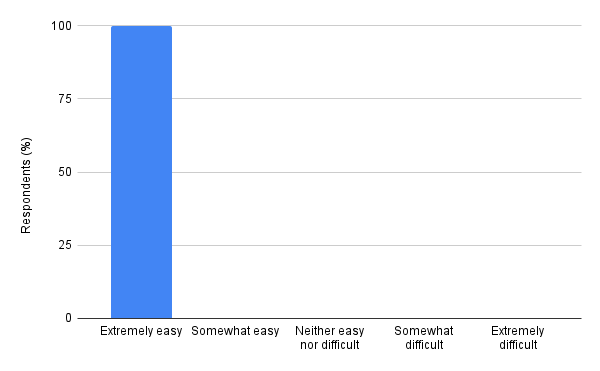
\includegraphics[width=0.75\textwidth]{10evaluation/images/stud1.png}
    \caption{Student participants responses concerning ease of posting a question.}
    \label{fig:stud1}
\end{figure}

\begin{figure}[H]
    \centering
    \textbf{2. Did you feel that you were aware of the demonstrators active presence on the system?}\par\medskip
    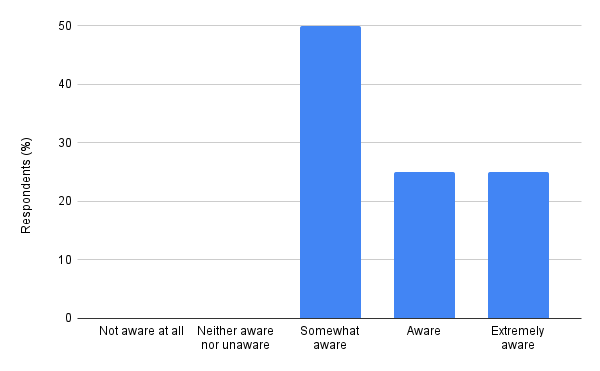
\includegraphics[width=0.75\textwidth]{10evaluation/images/stud2.png}
    \caption{Student participants responses concerning perceived awareness of demonstrators.}
    \label{fig:stud2}
\end{figure}

\begin{figure}[H]
    \centering
    \textbf{3. How satisfied were you with the `x people ahead of you in the queue' as a means of conveying wait time?}\par\medskip
    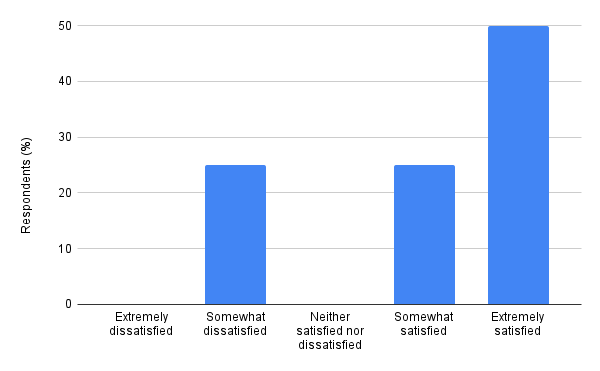
\includegraphics[width=0.75\textwidth]{10evaluation/images/stud3.png}
    \caption{Student participants responses concerning satisfaction with queue method.}
    \label{fig:stud3}
\end{figure}

\begin{figure}[H]
    \centering
    \textbf{4. How natural does the workflow, from posting a ticket to having the ticket marked as resolved, feel?}\par\medskip
    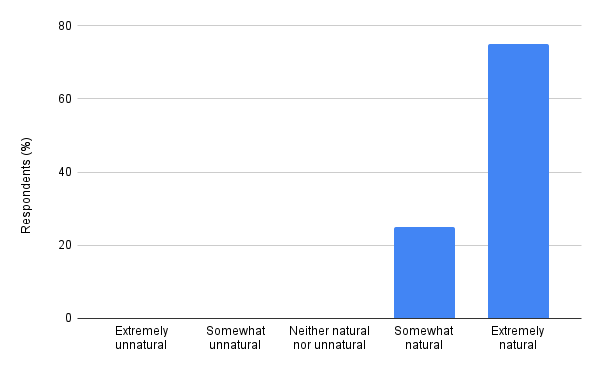
\includegraphics[width=0.75\textwidth]{10evaluation/images/stud4.png}
    \caption{Student participants responses concerning perceived naturalness of workflow.}
    \label{fig:stud4}
\end{figure}

\begin{figure}[H]
    \centering
    \textbf{5. How easy did you find using the video chat communications aspect of the system?}\par\medskip
    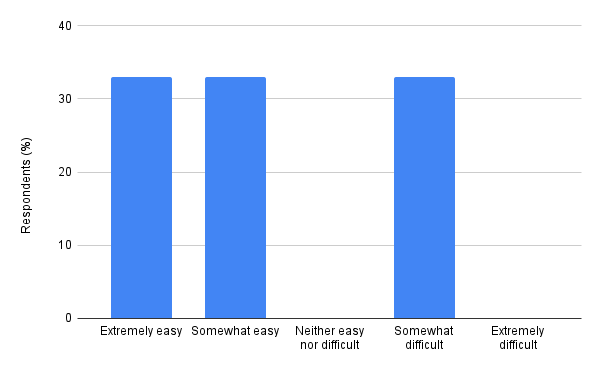
\includegraphics[width=0.75\textwidth]{10evaluation/images/stud5.png}
    \caption{Student participants responses concerning perceived ease of using video communication.}
    \label{fig:stud5}
\end{figure}

\begin{figure}[H]
    \centering
    \textbf{6. How easy did you find using the text chat communications aspect of the system?}\par\medskip
    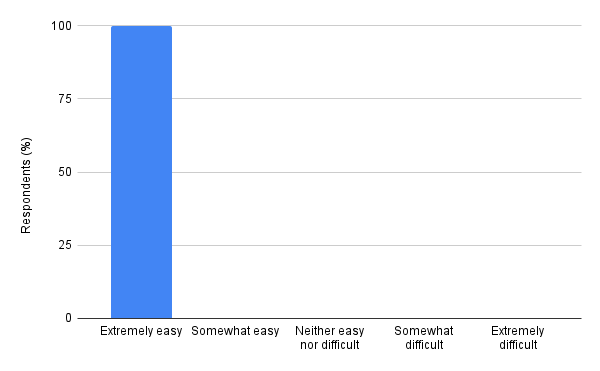
\includegraphics[width=0.75\textwidth]{10evaluation/images/stud6.png}
    \caption{Student participants responses concerning perceived ease of text chat communication.}
    \label{fig:stud6}
\end{figure}

\begin{figure}[H]
    \centering
    \textbf{7. How easy did you find using the file sharing communications aspect of the system?}\par\medskip
    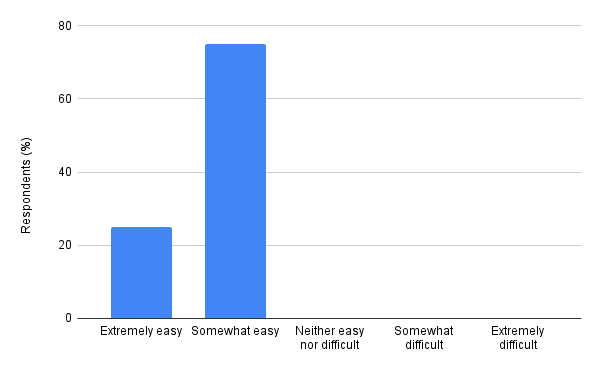
\includegraphics[width=0.75\textwidth]{10evaluation/images/stud7.png}
    \caption{Student participants responses concerning perceived ease of file sharing communication.}
    \label{fig:stud7}
\end{figure}

\begin{figure}[H]
    \centering
    \textbf{8. How easy did you find using the screensharing communications aspect of the system?}\par\medskip
    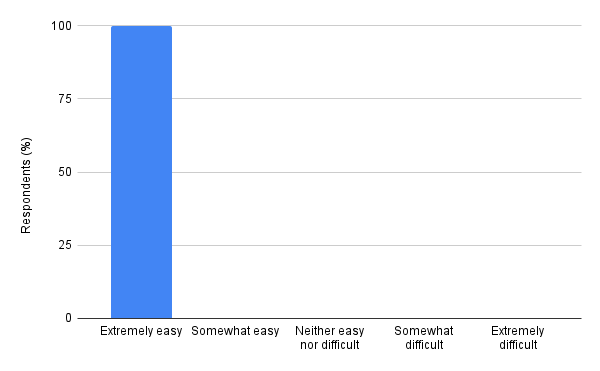
\includegraphics[width=0.75\textwidth]{10evaluation/images/stud8.png}
    \caption{Student participants responses concerning perceived ease screensharing sharing communication.}
    \label{fig:stud8}
\end{figure}

\textbf{9. Do you have any further notes or feedback on the communication aspect of system?}\par\medskip

The most notable pieces of non-positive feedback for this question were:

\begin{itemize}
    \item Consider breaking down the ticket posting form description field into "What's the problem", "What you've tried" and "Code".
    \item It might be useful to have the queue also display something like "there are currently N active sessions".
    \item For the file sharing, Ctrl+V or drag\&drop would be nice.
    \item It might be helpful to have hover over descriptions for the buttons, I was not sure what the arrow button under the call window did.
\end{itemize}

There was also a report of a `false start' with the video for one respondent. This issue has been addressed since the evaluation. Following the evaluation, all of the icon buttons had tooltips added to describe their function.

\textbf{10. Do you have any additional comments or suggestions on the ticket resolution workflow?}\par\medskip

The most notable pieces of non-positive feedback for this question were:

\begin{itemize}
    \item When waiting in the queue it would be nice to see how many lab leads are online in addition to the number of tickets in the queue.
    \item The ticket I posted was resolved, but I was surprised that I did not receive a success message, but got redirected to the starting page straight away.
    \item Have the "close ticket" box display that text in addition to the cross. I thought it would just close the session/window, and not the ticket itself. Possibly also color it green or red?	
\end{itemize}

Following the evaluation, the success message page was implemented as well as changing the `close ticket' icon box/button to a tick rather than a cross and a descriptive tooltip and colouring were added. 

\begin{figure}[H]
    \centering
    \textbf{11. How do you feel about the overall look and feel of the system?}\par\medskip
    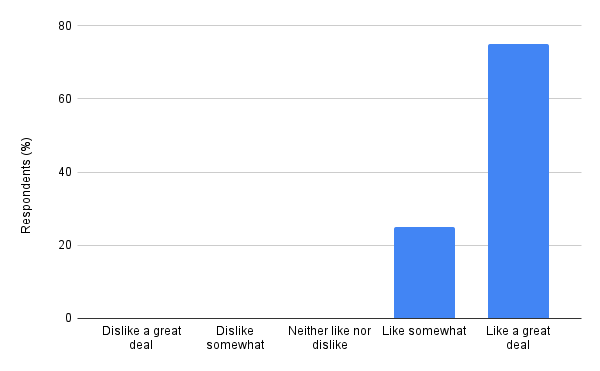
\includegraphics[width=0.75\textwidth]{10evaluation/images/stud11.png}
    \caption{Student participants responses concerning perceived look and feel of the system.}
    \label{fig:stud11}
\end{figure}

\begin{figure}[H]
    \centering
    \textbf{12. Overall, how easy would you say the system is to use?}\par\medskip
    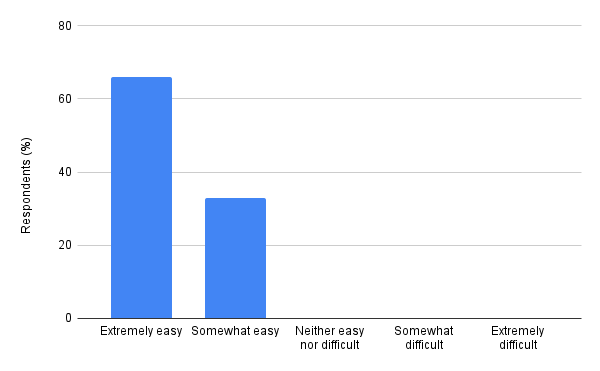
\includegraphics[width=0.75\textwidth]{10evaluation/images/stud12.png}
    \caption{Student participants responses concerning perceived overall ease of using the system.}
    \label{fig:stud12}
\end{figure}

\textbf{13. Do you have any further notes or feedback on the system?}\par\medskip

The most notable pieces of non-positive feedback for this question were:

\begin{itemize}
    \item One small remark: I was irritated by the input limit on the subject input field. I was trying to write a small description, something like "P1 - sayHello method of object syntax error", but only then figured that I was meant to write "P1" only.
    \item The chat window resizes awkwardly when starting a video call if the browser window is half-size of the screen. Might be worth resizing to the bottom in these cases.	
    \item The text input is limited for how my problem is called (Pract2), character limit at 6 was a bit confusing to describe my problem.
    \item For the problem description I would have liked some more guidance on what to type, such as "expected behaviour", "actual behaviour", or some questions that need to be answered, e.g. coding environment (might help? idk) in a field.
\end{itemize}

Following the evaluation, the limit on the `Practical' input field was increased. The chat window resizing was a key point, and should be noted for further work.

\subsubsection{Demonstrators}

Demonstrators also found the system easy to use, with all respondents finding it extremely easy to identify new tickets, assign themselves to tickets, initiate communication with the student, initiate a text chat and found it extremely or somewhat easy to initiate video calls and manage multiple tickets at once. The solution providing aspect of the system had more mixed results, with half of the participants finding it extremely easy but the other half finding it neither easy nor difficult. Demonstrators appreciated the overall system, with all respondents finding the workflow extremely natural, codeHelper `much better' than the current system, extremely easy to use overall and said they were somewhat satisfied with the overall look and feel.

For the 4 participants acting as demonstrators, the questionnaire responses are given below. 

\begin{figure}[H]
    \centering
    \textbf{1. How easy did you find it to identify a new, open ticket?}\par\medskip
    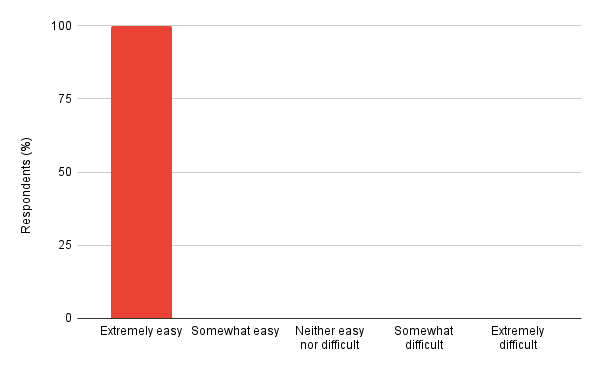
\includegraphics[width=0.75\textwidth]{10evaluation/images/dem1.png}
    \caption{Demonstrator participants responses concerning perceived ease of identifying new, live tickets.}
    \label{fig:dem1}
\end{figure}

\begin{figure}[H]
    \centering
    \textbf{2. How easy did you find it to assign a ticket to yourself?}\par\medskip
    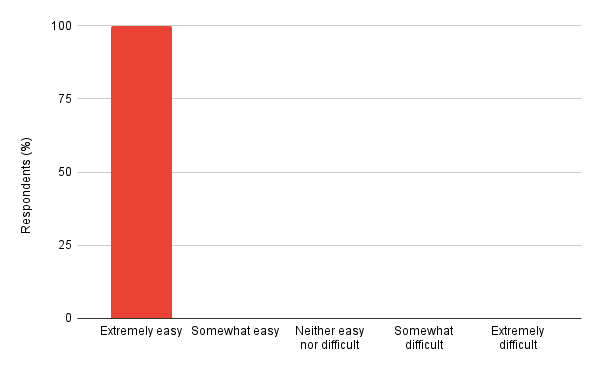
\includegraphics[width=0.75\textwidth]{10evaluation/images/dem2.png}
    \caption{Demonstrator participants responses concerning perceived ease of assigning themselves to a ticket.}
    \label{fig:dem2}
\end{figure}

\begin{figure}[H]
    \centering
    \textbf{3. How easy did you find it to initiate communication with the student?}\par\medskip
    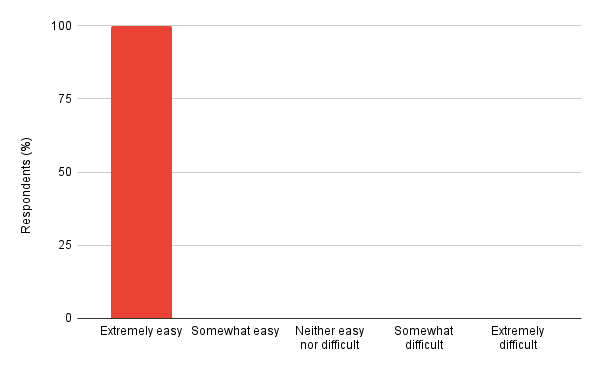
\includegraphics[width=0.75\textwidth]{10evaluation/images/dem3.png}
    \caption{Demonstrator participants responses concerning perceived ease of initiating communication with a student.}
    \label{fig:dem3}
\end{figure}

\begin{figure}[H]
    \centering
    \textbf{4. How easy did you find it to initiate a text chat?}\par\medskip
    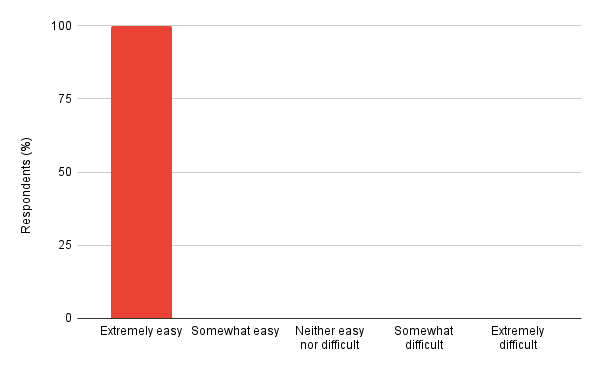
\includegraphics[width=0.75\textwidth]{10evaluation/images/dem4.png}
    \caption{Demonstrator participants responses concerning perceived ease of initiating a text chat.}
    \label{fig:dem4}
\end{figure}

\begin{figure}[H]
    \centering
    \textbf{5. How easy did you find it to initiate a video chat?}\par\medskip
    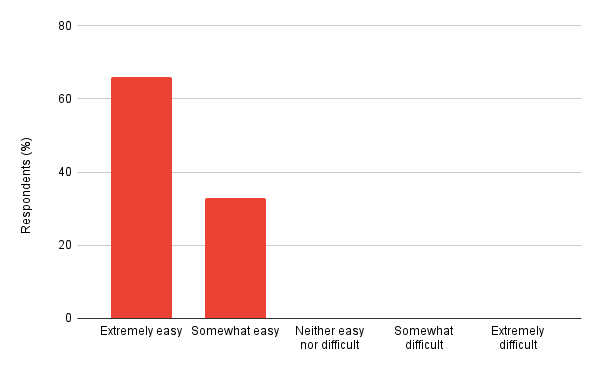
\includegraphics[width=0.75\textwidth]{10evaluation/images/dem5.png}
    \caption{Demonstrator participants responses concerning perceived ease of initiating video communication.}
    \label{fig:dem5}
\end{figure}

\begin{figure}[H]
    \centering
    \textbf{6. How easy did you find it to manage multiples tickets and chats at the same time?}\par\medskip
    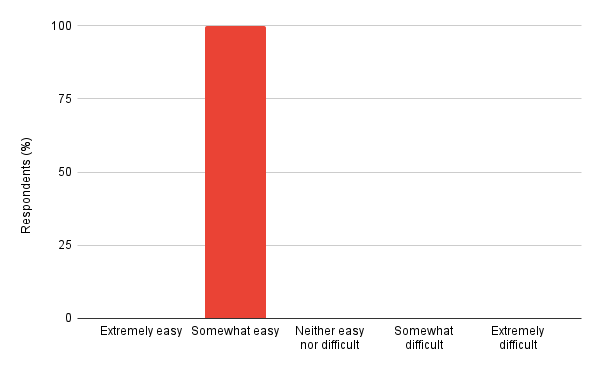
\includegraphics[width=0.75\textwidth]{10evaluation/images/dem6.png}
    \caption{Demonstrator participants responses concerning perceived ease of managing multiple tickets at once.}
    \label{fig:dem6}
\end{figure}

\begin{figure}[H]
    \centering
    \textbf{8. How easy did you find the solution providing aspect of the system?}\par\medskip
    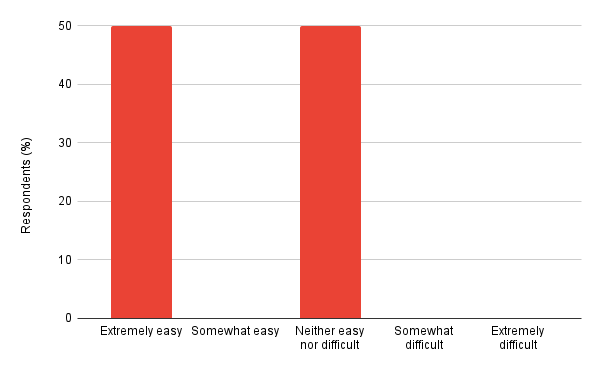
\includegraphics[width=0.75\textwidth]{10evaluation/images/dem8.png}
    \caption{Demonstrator participants responses concerning perceived ease of using the solution providing aspect of the system.}
    \label{fig:dem8}
\end{figure}

\textbf{10. Do you have any further notes or feedback on the communication aspect of system?}\par\medskip

The most notable pieces of non-positive feedback for this question were:

\begin{itemize}
    \item Have the "close ticket" button display that text along with the 'X'. I thought it would close the current window/chat rather than the whole ticket. Maybe also colour it green or red?	
\end{itemize}

\begin{figure}[H]
    \centering
    \textbf{16. How natural does the workflow, from a new ticket being posted to marking the ticket as resolved and posting a solution, feel?}\par\medskip
    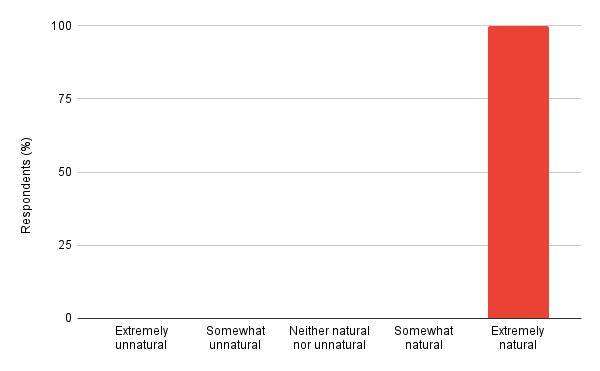
\includegraphics[width=0.75\textwidth]{10evaluation/images/dem(2)1.png}
    \caption{Demonstrator participants responses concerning perceived naturalness of workflow.}
    \label{fig:dem16}
\end{figure}

\begin{figure}[H]
    \centering
    \textbf{18. How does the system compare to the current form/list/teams based solution?}\par\medskip
    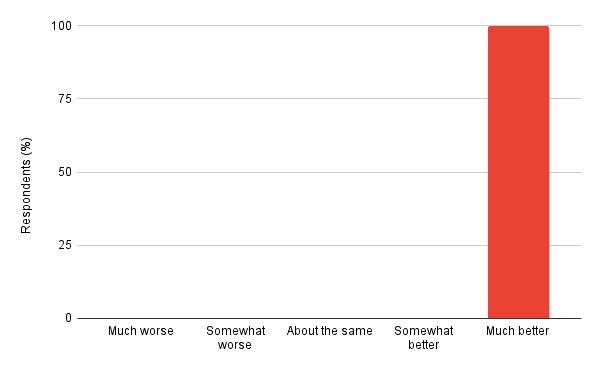
\includegraphics[width=0.75\textwidth]{10evaluation/images/dem(2)3.png}
    \caption{Demonstrator participants responses concerning perceived relative comparison with current system.}
    \label{fig:dem18}
\end{figure}

\begin{figure}[H]
    \centering
    \textbf{19. How do you feel about the overall look and feel of the system?}\par\medskip
    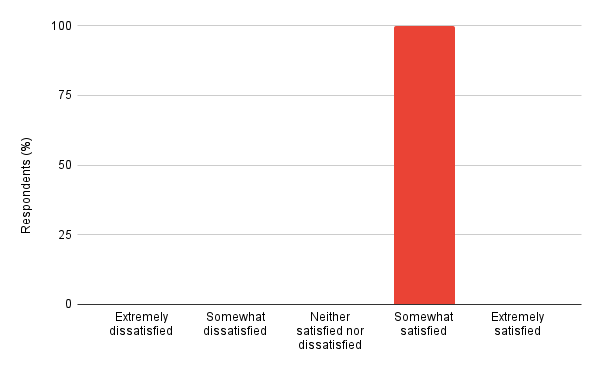
\includegraphics[width=0.75\textwidth]{10evaluation/images/dem(2)4.png}
    \caption{Demonstrator participants responses concerning perceived look and feel of the system.}
    \label{fig:dem19}
\end{figure}

\begin{figure}[H]
    \centering
    \textbf{29. Overall, how easy would you say the system is to use?}\par\medskip
    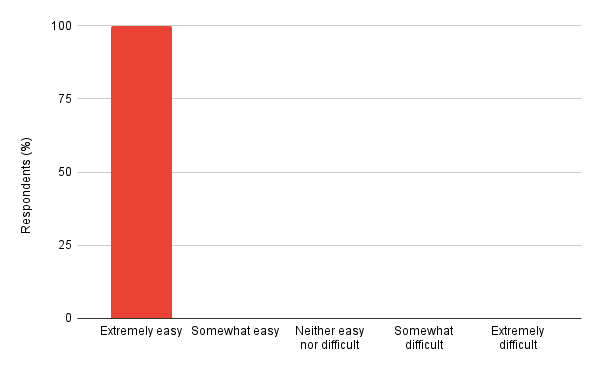
\includegraphics[width=0.75\textwidth]{10evaluation/images/dem(2)5.png}
    \caption{Demonstrator participants responses concerning perceived overall ease of using the system.}
    \label{fig:dem29}
\end{figure}

\subsection{Discussion} \label{sec:discusseval}

In this section, the results of the experiment are discussed and used to evaluate the design choices against Lauesen's usability factors \cite{lauesen} that were outlined as the design objectives of the application (discussed in section \ref{sec:interface}).

\subsubsection{Lauesen's Usability Factors}

    \paragraph{Fit for Use} From the student's perspective, the system appears to support the tasks that the user has in real life. 100\% of respondents found posting a question, using screensharing and using livechat `extremely easy', 75\% found the workflow extremely natural and 25\% found it somewhat natural, the majority of users found the video chat at least somewhat easy (and the response that it was `somewhat difficult' is likely related to the bug that was reported and fixed) and 100\% of respondents found file sharing at least `somewhat easy'.
    From the demonstrator's perspective, the system (again) appears to support the tasks. 100\% of respondents found it easy to identify new tickets, assign themselves to tickets, initiate communication, initiate a text chat specifically and also to use the system overall. 100\% of respondents found it at least somewhat easy to initiate a video chat and 100\% of respondents found managing multiple tickets/chats simultaneously somewhat easy. 
    The actions discussed above are all of the key components required by participants to communicate with others and work to resolve issues, the task that the system is to support.
    
    \paragraph{Ease of Learning, Remembering and Understandability} 100\% of demonstrators and 66\% of students found the overall system extremely easy to use, with the remaining 33\% of students finding it somewhat easy. This response is after a first use of the system in a 20 minute test, with no training or instruction of how to use the system.
    
    \paragraph{Task Efficiency} For students, 75\% of respondents found the workflow extremely natural, with the remaining 25\% finding it somewhat natural. 
    For demonstrators, 100\% found the workflow extremely natural and found managing multiple tickets/chats somewhat easy. 
    These responses, alongside previously discussed ease and satisfaction responses to communication, would appear to suggest that participants found the process to be efficient. One thing to note is that 50\% of respondents found the solution aspect of the system neither easy nor difficult - if this aspect of the system were to be improved then it would increase efficiency by increasing demonstrators use of the reusable solutions.
    
    \paragraph{Subjective Satisfaction} 100\% of demonstrator respondents were somewhat satisfied with the overall look and feel of the system, 75\% of student respondents were extremely satisfied and 25\% were somewhat satisfied. 
    These responses suggest that users were satisfied with the overall system. Although there is room for improvement on this front, it is likely related to the fact that the system was built under time constraints and is more a proof-of-concept than production build - future work on `tidying' some of the features as well as greater experience using the system in practice would reveal opportunities to improve user satisfaction.

\subsubsection{Notes}

Note that some questions were omitted from the evaluation discussion as they did not receive any responses.

Questions regarding the summary and statistics section did not receive any responses. This is likely because, although given lab lead privileges in order to view the section, the volunteers were acting as demonstrators and had knowledge and experience in this area. As a result, they did not seek out the statistics section because they would not in real life. Additionally, the statistics section only contained the small amount of data collected in the experiment and therefore did not provide much insight.

Questions regarding `non-responsive students' were also not answered. This is likely resulting from the fact that no demonstrator had experience with non-responsive students during the experiment.

\newpage
\section{Customer Feedback} 

The customer, dissertation supervisor, provided the following feedback:

``\textit{System does exactly what I was hoping for. I am very pleased the video/screenshare functionality was integrated into the webapp. Overall, it provides a much slicker and neater way of managing labs. The statistics are a great addition. The one change/addition I would like, is to be able to select which graphs to display and to be able to export the graphs/data. Also, I would have liked a prompt before closing a ticket to enter a solution if one had not been provided.}''

\newpage
\section{Google Lighthouse}

Google Lighthouse \cite{Lighthouse} was also used to evaluate the application. Google Lighthouse is tool that runs a series of audits of sites which produce reports, analysing five categories: web accessibility, best practices, web performance, search engine optimization, and progressive web applications.

The Lighthouse scores are shown in figure \ref{fig:lighthouse}.

\begin{figure}[H]
    \centering
    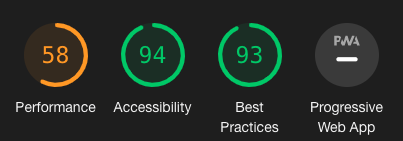
\includegraphics[width=0.5\textwidth]{10evaluation/images/lighthouse.png}
    \caption{Google Lighthouse scores for evaluation of the codeHelper application.}
    \label{fig:lighthouse}
\end{figure}

The aspects which most detriment performance are discussed in the limitations and future work section, \ref{sec:futurework}.

\newpage
\section{Comparing Existing Tools with codeHelper}

In this section, the existing tools analysed in Chapter \ref{chap:context} shall be compared to the developed codeHelper system.  

Table \ref{tab:comparetools} shows a side-by-side comparison of codeHelper, Spiceworks and ClassroomQ against the requirements outlined in chapter \ref{chap:req}. 

\begin{table}[H]
    \centering
    \begin{tabular}{c|c|c|c|c}
        & & codeHelper & Spiceworks & ClassroomQ \\
        \hline\hline
         F-01 & Users can Register & \color{green} \textbf{ \color{green} \textbf{\checked}} &  \color{green} \textbf{\checked} &  \color{green} \textbf{\checked} \\
         \hline
         F-02 & Users can Login with Shibboleth  & \color{red} \textbf{x}  & \color{red} \textbf{x}  & \color{red} \textbf{x} \\
         \hline
         F-03 & Admin can assign roles &  \color{green} \textbf{\checked} &  \color{green} \textbf{\checked}  & \color{red} \textbf{x} \\
         \hline
         F-04 & Users can Login/Logout &  \color{green} \textbf{\checked} &  \color{green} \textbf{\checked} &  \color{green} \textbf{\checked} \\
         \hline
         F-05 & Students can post tickets with info &  \color{green} \textbf{\checked} &  \color{green} \textbf{\checked}  & \color{red} \textbf{x} \\
          \hline
         F-06 & Students can add tags &  \color{green} \textbf{\checked}  & \color{red} \textbf{x}  & \color{red} \textbf{x} \\
          \hline
         F-07 & System recommends similar tickets  & \color{red} \textbf{x}  & \color{red} \textbf{x}  & \color{red} \textbf{x} \\
          \hline
         F-08 & Tracks selected ticket recommendation  & \color{red} \textbf{x}  & \color{red} \textbf{x}  & \color{red} \textbf{x} \\
          \hline
         F-09 & Demonstrator can assign self to ticket &  \color{green} \textbf{\checked} &  \color{green} \textbf{\checked}  & \color{red} \textbf{x} \\
          \hline
         F-10 & Demonstrator can chat on own tickets &  \color{green} \textbf{\checked}  & \color{red} \textbf{x}  & \color{red} \textbf{x} \\
          \hline
         F-11 & Demonstrator can close ticket &  \color{green} \textbf{\checked} &  \color{green} \textbf{\checked}  & \color{red} \textbf{x} \\
          \hline
         F-12 & Student can close ticket &  \color{green} \textbf{\checked}  & \color{red} \textbf{x}  & \color{red} \textbf{x} \\
          \hline
         F-13 & Lablead can open and close labs &  \color{green} \textbf{\checked}  & \color{red} \textbf{x}  & \color{red} \textbf{x} \\
          \hline
         F-14 & Lablead can disable accounts  & \color{red} \textbf{x}  & \color{red} \textbf{x}  & \color{red} \textbf{x} \\
          \hline
         F-15 & System prevents offensive content  & \color{red} \textbf{x}  & \color{red} \textbf{x}  & \color{red} \textbf{x} \\
          \hline
         F-16 & System allows users 1 live ticket &  \color{green} \textbf{\checked}  & \color{red} \textbf{x}  & \color{red} \textbf{x} \\
          \hline
         F-17 & Students can edit their live ticket  & \color{red} \textbf{x}  & \color{red} \textbf{x}  & \color{red} \textbf{x} \\
          \hline
         F-18 & Demonstrator can livechat on all tickets &  \color{green} \textbf{\checked}  & \color{red} \textbf{x}  & \color{red} \textbf{x} \\
        \hline
         F-19 & Users can video call &  \color{green} \textbf{\checked}  & \color{red} \textbf{x}  & \color{red} \textbf{x} \\
                 \hline
         F-20a & Demonstrator can create reusable solution &  \color{green} \textbf{\checked}  & \color{red} \textbf{x}  & \color{red} \textbf{x} \\
                 \hline
         F-20b & Demonstrator can edit existing solution &  \color{green} \textbf{\checked}  & \color{red} \textbf{x}  & \color{red} \textbf{x} \\
                 \hline
         F-20c & Demonstrator can assign solution to ticket &  \color{green} \textbf{\checked}  & \color{red} \textbf{x}  & \color{red} \textbf{x} \\
                 \hline
         F-21 & System prompts for solution to problems  & \color{red} \textbf{x}  & \color{red} \textbf{x}  & \color{red} \textbf{x} \\
                 \hline
         F-22 & Demonstrator can livechat on all tickets &  \color{green} \textbf{\checked}  & \color{red} \textbf{x} &  \color{green} \textbf{\checked} \\
                 \hline
         F-23 & User can specify in-person location &  \color{green} \textbf{\checked} &  \color{green} \textbf{\checked} &  \color{green} \textbf{\checked} \\
            \hline
         F-24 & User can send files &  \color{green} \textbf{\checked}  & \color{red} \textbf{x}  & \color{red} \textbf{x} \\
            \hline
         F-25 & System shows timeline of actions &  \color{green} \textbf{\checked} &  \color{green} \textbf{\checked}  & \color{red} \textbf{x} \\
            \hline
         F-26 & System shows statistics by lab &  \color{green} \textbf{\checked}  & \color{red} \textbf{x}  & \color{red} \textbf{x} \\
            \hline
          F-26 & System shows statistics by class &  \color{green} \textbf{\checked}  & \color{red} \textbf{x}  & \color{red} \textbf{x} \\
            \hline
    \end{tabular}
    \caption{Comparison of functional system requirements achieved by codeHelper, Spiceworks and ClassroomQ systems.}
    \label{tab:comparetools}
\end{table}

